\section{LatentMoE Core Design Principles}\label{sec:design_choices}
 
Before delving into the specifics of LatentMoE, we first take a systems-level view of what is required to deploy an MoE model that is both accurate and cost-efficient.

Throughout this section, we use Qwen3-235B-A22B as a running example for our modeling, with 
$N = 128$ experts, $K=8$ active experts per token, a hidden dimension $d=4096$, and an intermediate feed-forward dimension $m=1536$. For concreteness, we consider deployment on NVIDIA GB200 GPUs interconnected by a high-bandwidth NVLink fabric, which provides approximately $1800$~GB/s of bidirectional bandwidth per GPU (i.e., $\nvlinkbw=900$~GB/s per direction). To ensure that expert communication remains within a single NVLink domain, experts are distributed via expert parallelism across $\ep=64$ GPUs. Attention layers are executed using data parallelism over the same group of GPUs. Each GB200 GPU delivers a peak FP4 Tensor Core throughput of $F=10$ PFLOPs and an HBM memory bandwidth of $\hbmbw=8$~TB/s \citep{nvidia_blackwell}.

\subsection{Memory Bandwidth Bottleneck}
In highly interactive (\ie, low-latency) settings that typically use small batch sizes, MoE computation is primarily bottlenecked by memory bandwidth. Figure~\ref{fig:roofline} provides a high-level roof-line analysis of performance versus arithmetic intensity.

\begin{figure}[ht!]
    \centering
    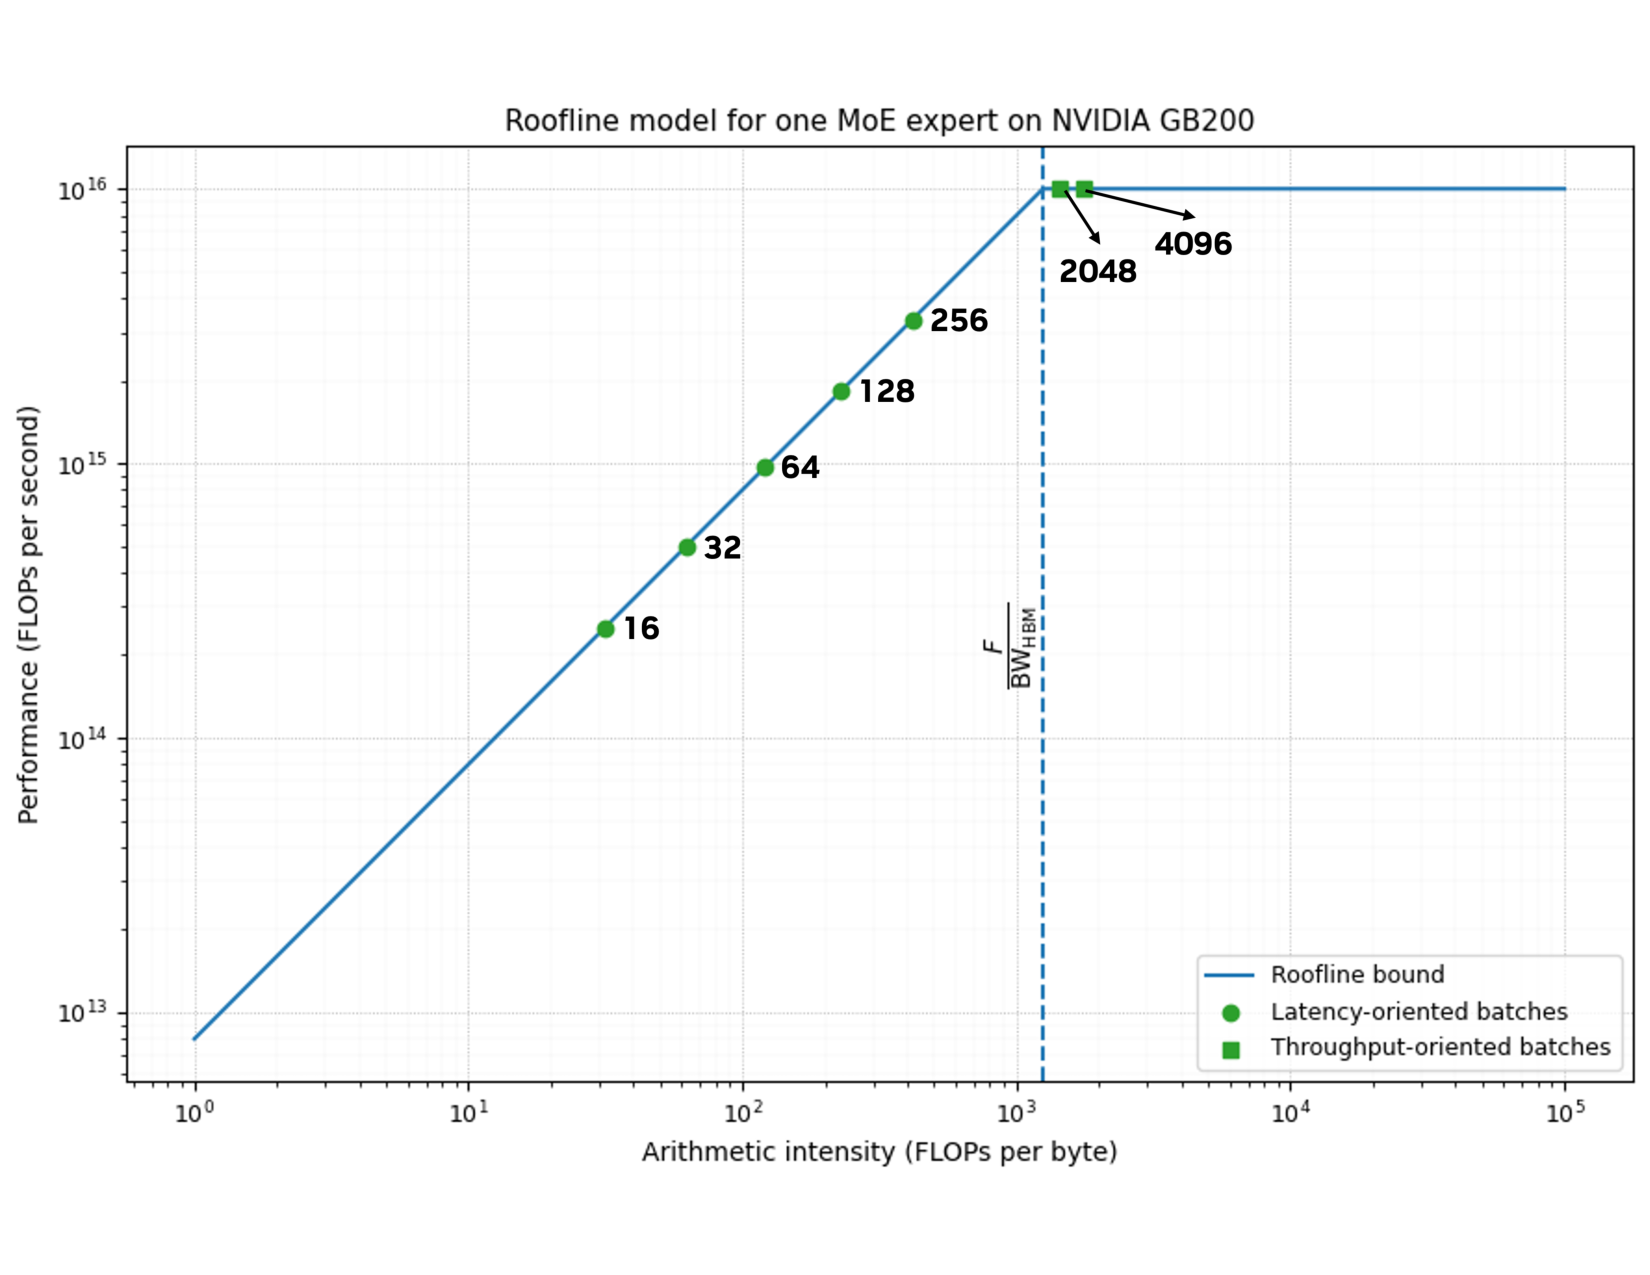
\includegraphics[width=0.7\linewidth]{figures/roofline_moe_qwen235b_clean.pdf}
    \caption{\textbf{Roofline Analysis for serving Qwen3-235B-A22B.}
    Operating points correspond to different per-expert token counts $\texp$ (i.e., effective expert batch sizes after MoE routing), mapped to arithmetic intensity $I=\frac{2 \cdot \texp \cdot d \cdot m}{d \cdot m + \texp \cdot (d+m)}$. At latency-critical batch sizes (low $I$), MoE expert computation is constrained by HBM bandwidth rather than compute, and the operating points lie in the bandwidth-bound regime.}
    \label{fig:roofline}
\end{figure}

For a GB200 system, a computation becomes compute-bound only if its arithmetic intensity (i.e., FLOPs per byte) exceeds:
\begin{equation*}
\frac{F}{\hbmbw} = \frac{10 \times 10^{15}}{8 \times 10^{12}} = 1250 \text{ FLOPs/byte}.
\end{equation*}

Let $\ttotal$ be the total number of tokens across the $\ep$ GPUs prior to MoE routing. Assuming a uniform distribution of tokens across experts, the number of tokens assigned to a single expert is: $\texp := \frac{\ttotal \cdot K}{N}$. In the Qwen3-235B-A22B example, with $N = 128$ and $\ep = 64$, each GPU hosts $N / \ep = 2$ experts; thus each GPU processes approximately $2 \cdot \texp$ expert tokens per MoE layer.

The FP4 compute cost for a single expert is $C_{\mathrm{exp}} = 2 \cdot \texp \cdot d \cdot m$, and the corresponding memory traffic in FP4 precision---accounting for weights, inputs, and intermediate activations---is given by $M_{\mathrm{exp}} = d \cdot m + \texp \cdot (d + m)$. Since each GPU processes two experts in our example, the arithmetic intensity $I$ is given by the ratio of the total compute to the total memory traffic:
\begin{equation*}
I = \frac{2 \cdot C_{\mathrm{exp}}}{2 \cdot M_{\mathrm{exp}}} = \frac{2 \cdot \texp \cdot d \cdot m}{d \cdot m + \texp \cdot (d + m)}.
\end{equation*}
To operate in the compute-bound regime, we require $I \ge 1250$. Substituting the Qwen3-235B-A22B parameters yields the condition:
\begin{equation*}
\frac{2 \cdot \texp \cdot d \cdot m}{d \cdot m + \texp \cdot (d + m)} \ge 1250 \quad \implies \quad \texp \ge 1418.
\end{equation*}
In typical latency-critical deployments, effective batch sizes are small, resulting in $\texp$ being on the order of a few hundred tokens—well below the threshold of 1418. Consequently, MoE experts operate in the memory-bound region of the roofline curve (Figure~\ref{fig:roofline}), where performance is limited by weight loading rather than compute capacity.

\begin{notebox}{Design Principle I}
In low-latency serving scenarios, MoE inference is typically dominated by the memory-bandwidth cost of loading model weights. Consequently, maximizing accuracy per parameter is critical for applications with high interactivity requirements.
\end{notebox}


\subsection{Communication Bottleneck}
In throughput-oriented settings, once experts become compute-bound, communication emerges as a significant contributor to end-to-end execution time in distributed settings. Expert parallelism mandates all-to-all token routing across devices, imposing an overhead that can control end-to-end execution time.
Recall that in our example configuration, each GPU hosts two experts. Since $\texp$ denotes the tokens processed per expert, each GPU processes a total of $2 \texp$ tokens across its local experts per MoE layer.

Assuming a uniform distribution of tokens, the all-to-all communication volume per GPU per MoE layer is given by:
\begin{equation*}
M_{\mathrm{comm}} = 2.5 \cdot \left( \frac{N}{\ep} \cdot \texp \cdot d \right) = 5 \cdot \texp \cdot d.
\end{equation*}
Here, the factor 2.5 accounts for the mixed-precision traffic (0.5 bytes for FP4 dispatch, 2 bytes for BF16 aggregation). On the compute side, the total FLOP count for the two local experts is:
\begin{equation*}
C_{\mathrm{comp}} = 2 \cdot \left( \frac{N}{\ep} \cdot \texp \cdot d \cdot m \right) = 4 \cdot \texp \cdot d \cdot m.
\end{equation*}
The corresponding compute time is: $t_{\mathrm{comp}} = \frac{C_{\mathrm{comp}}}{F} = \frac{4 \cdot \texp \cdot d \cdot m}{F}$. Similarly, the all-to-all communication time is:
$t_{\mathrm{comm}} = \frac{M_{\mathrm{comm}}}{\mathrm{BW}_{\mathrm{NVL}}} = \frac{5 \cdot \texp \cdot d}{\mathrm{BW}_{\mathrm{NVL}}}$,
where $\mathrm{BW}_{\mathrm{NVL}} = 900~\text{GB/s}$ is the effective unidirectional NVLink bandwidth. Consequently, the ratio of communication time to compute time is:
\begin{equation*}
\frac{t_{\mathrm{comm}}}{t_{\mathrm{comp}}} = \frac{5 \cdot \texp \cdot d / \mathrm{BW}_{\mathrm{NVL}}}{4 \cdot \texp \cdot d \cdot m / F} = \frac{5 \cdot F}{4 \cdot m \cdot \, \mathrm{BW}_{\mathrm{NVL}}}.
\end{equation*}
Substituting the parameters for the GB200 NVL72 and Qwen3-235B-A22B yields a ratio of approximately 9. This indicates that in the throughput-oriented regime, MoE layers are heavily dominated by all-to-all communication overhead.

\begin{notebox}{Design Principle II}
Improving performance in throughput-oriented MoE deployments requires minimizing the data volume of all-to-all operations. This volume is proportional to:
\begin{equation*}
M_{\mathrm{comm}} \propto \frac{N}{\ep} \cdot \texp \cdot d = \frac{\ttotal \cdot K \cdot d}{\ep}.
\end{equation*}
Consequently, communication overhead can be mitigated by reducing the routed hidden dimension $d$ or the number of active experts $K$. Note that modifying the intermediate dimension $m$ does not affect the token size and thus yields no direct improvement.
\end{notebox}

\subsection{Model Quality}
Beyond optimizing inference speed, preserving model quality is paramount. To this end, we draw on theoretical insights into neural network expressivity and combinatorial sparsity.
Classical results on Barron functions~\citep{barron1993} state that a one-hidden-layer network with $u$ nonlinear units achieves a mean-squared error of $\mathcal{O}(1/u)$, independent of the input dimension $d$. In an MoE layer, this effective nonlinear budget per token is proportional to the total width of the selected experts:
\begin{equation*}
U_{\mathrm{eff}} \propto K \cdot m.
\end{equation*}
This implies that reducing the active experts $K$ or the intermediate dimension $m$ directly penalizes the effective capacity ($U_{\mathrm{eff}}$), risking model quality degradation.

\begin{notebox}{Design Principle III}
Maintaining model quality requires preserving the effective nonlinear budget, $K \cdot m$. Consequently, to alleviate memory and communication bottlenecks without sacrificing model quality, we should keep both the number of active experts and the intermediate dimension unchanged.
\end{notebox}

Every inference task is characterized by an intrinsic feature rank, $r_\mathrm{eff}$, corresponding to the minimum number of degrees of freedom required to preserve task-relevant information. Reducing the hidden dimension $d$ below this threshold necessarily discards such information, leading to accuracy degradation. Thus, $r_\mathrm{eff}$ serves as a task-dependent lower bound on $d$.

\begin{notebox}{Design Principle IV}
There exists a task-specific feature rank $r_\mathrm{eff}$ that imposes a lower limit on the reduction of $d$. Reducing $d$ below this limit precipitates a collapse in model quality.
\end{notebox}

Additionally, the MoE architecture benefits from combinatorial sparsity, offering $\binom{N}{K}$ possible expert combinations per token~\citep{deepseekmoe}. Increasing the total number of experts $N$ expands this specialization space. Furthermore, scaling both $N$ and $K$ by a factor $\alpha$ exponentially increases the diversity of expert mixtures:
\begin{equation*}
    \binom{\alpha N}{\alpha K} \ge \left( \binom{N}{K} \right)^\alpha.
\end{equation*}

\begin{notebox}{Design Principle V}
Scaling both the number of experts $N$ and top-k per token $K$ enhances model quality by exponentially expanding the space of expert combinations.
\end{notebox}

\paragraph{Putting it all together.} Design Principles I and II indicate that improving inference speed requires reducing both memory bandwidth and communication costs. Memory bandwidth cost scales with 
$d$ and $m$, while communication cost scales with $K$ and $d$. However, Principle III cautions against reducing either $K$ or $m$, as doing so would likely degrade model quality. This leaves $d$ as the most promising dimension to reduce, enabling performance improvements in both throughput- and latency-oriented regimes without significant loss in accuracy. Principle IV further establishes a lower bound, ($r_\mathrm{eff}$), on $d$ to prevent quality collapse. Moreover, Principle V suggests that increasing $N$ and $K$ improves model quality. Since memory bandwidth and communication costs scale linearly with $K$, we can simultaneously increase $K$ by a factor $\alpha$ and reduce $d$ by the same factor $\alpha$ (provided $d/\alpha \ge r_\mathrm{eff}$). \textcolor{green!50!black}{\textit{We hypothesize, and empirically validate in subsequent sections, that this transformation (also depicted in Figure~\ref{fig:latent_moe}) preserves memory bandwidth and communication costs while improving network expressivity and combinatorial sparsity, yielding higher accuracy per FLOP and per parameter.}}
